\documentclass[twoside]{book}

% Packages required by doxygen
\usepackage{fixltx2e}
\usepackage{calc}
\usepackage{doxygen}
\usepackage[export]{adjustbox} % also loads graphicx
\usepackage{graphicx}
\usepackage[utf8]{inputenc}
\usepackage{makeidx}
\usepackage{multicol}
\usepackage{multirow}
\PassOptionsToPackage{warn}{textcomp}
\usepackage{textcomp}
\usepackage[nointegrals]{wasysym}
\usepackage[table]{xcolor}

% NLS support packages
\usepackage{polski}
\usepackage[T1]{fontenc}

% Font selection
\usepackage[T1]{fontenc}
\usepackage[scaled=.90]{helvet}
\usepackage{courier}
\usepackage{amssymb}
\usepackage{sectsty}
\renewcommand{\familydefault}{\sfdefault}
\allsectionsfont{%
  \fontseries{bc}\selectfont%
  \color{darkgray}%
}
\renewcommand{\DoxyLabelFont}{%
  \fontseries{bc}\selectfont%
  \color{darkgray}%
}
\newcommand{\+}{\discretionary{\mbox{\scriptsize$\hookleftarrow$}}{}{}}

% Page & text layout
\usepackage{geometry}
\geometry{%
  a4paper,%
  top=2.5cm,%
  bottom=2.5cm,%
  left=2.5cm,%
  right=2.5cm%
}
\tolerance=750
\hfuzz=15pt
\hbadness=750
\setlength{\emergencystretch}{15pt}
\setlength{\parindent}{0cm}
\setlength{\parskip}{3ex plus 2ex minus 2ex}
\makeatletter
\renewcommand{\paragraph}{%
  \@startsection{paragraph}{4}{0ex}{-1.0ex}{1.0ex}{%
    \normalfont\normalsize\bfseries\SS@parafont%
  }%
}
\renewcommand{\subparagraph}{%
  \@startsection{subparagraph}{5}{0ex}{-1.0ex}{1.0ex}{%
    \normalfont\normalsize\bfseries\SS@subparafont%
  }%
}
\makeatother

% Headers & footers
\usepackage{fancyhdr}
\pagestyle{fancyplain}
\fancyhead[LE]{\fancyplain{}{\bfseries\thepage}}
\fancyhead[CE]{\fancyplain{}{}}
\fancyhead[RE]{\fancyplain{}{\bfseries\leftmark}}
\fancyhead[LO]{\fancyplain{}{\bfseries\rightmark}}
\fancyhead[CO]{\fancyplain{}{}}
\fancyhead[RO]{\fancyplain{}{\bfseries\thepage}}
\fancyfoot[LE]{\fancyplain{}{}}
\fancyfoot[CE]{\fancyplain{}{}}
\fancyfoot[RE]{\fancyplain{}{\bfseries\scriptsize Wygenerowano przez Doxygen }}
\fancyfoot[LO]{\fancyplain{}{\bfseries\scriptsize Wygenerowano przez Doxygen }}
\fancyfoot[CO]{\fancyplain{}{}}
\fancyfoot[RO]{\fancyplain{}{}}
\renewcommand{\footrulewidth}{0.4pt}
\renewcommand{\chaptermark}[1]{%
  \markboth{#1}{}%
}
\renewcommand{\sectionmark}[1]{%
  \markright{\thesection\ #1}%
}

% Indices & bibliography
\usepackage{natbib}
\usepackage[titles]{tocloft}
\setcounter{tocdepth}{3}
\setcounter{secnumdepth}{5}
\makeindex

% Hyperlinks (required, but should be loaded last)
\usepackage{ifpdf}
\ifpdf
  \usepackage[pdftex,pagebackref=true]{hyperref}
\else
  \usepackage[ps2pdf,pagebackref=true]{hyperref}
\fi
\hypersetup{%
  colorlinks=true,%
  linkcolor=blue,%
  citecolor=blue,%
  unicode%
}

% Custom commands
\newcommand{\clearemptydoublepage}{%
  \newpage{\pagestyle{empty}\cleardoublepage}%
}

\usepackage{caption}
\captionsetup{labelsep=space,justification=centering,font={bf},singlelinecheck=off,skip=4pt,position=top}

%===== C O N T E N T S =====

\begin{document}

% Titlepage & ToC
\hypersetup{pageanchor=false,
             bookmarksnumbered=true,
             pdfencoding=unicode
            }
\pagenumbering{alph}
\begin{titlepage}
\vspace*{7cm}
\begin{center}%
{\Large TM \\[1ex]\large 1 }\\
\vspace*{1cm}
{\large Wygenerowano przez Doxygen 1.8.13}\\
\end{center}
\end{titlepage}
\clearemptydoublepage
\pagenumbering{roman}
\tableofcontents
\clearemptydoublepage
\pagenumbering{arabic}
\hypersetup{pageanchor=true}

%--- Begin generated contents ---
\chapter{Indeks przestrzeni nazw}
\section{Pakiety}
Oto lista pakietów wraz z krótkim opisem (o ile jest dostępny)\+:\begin{DoxyCompactList}
\item\contentsline{section}{\hyperlink{namespace_steganografia_t_m}{Steganografia\+TM} }{\pageref{namespace_steganografia_t_m}}{}
\end{DoxyCompactList}

\chapter{Indeks hierarchiczny}
\section{Hierarchia klas}
Ta lista dziedziczenia posortowana jest z grubsza, choć nie całkowicie, alfabetycznie\+:\begin{DoxyCompactList}
\item Form\begin{DoxyCompactList}
\item \contentsline{section}{Steganografia\+T\+M.\+O\+K\+NO}{\pageref{class_steganografia_t_m_1_1_o_k_n_o}}{}
\end{DoxyCompactList}
\end{DoxyCompactList}

\chapter{Indeks struktur danych}
\section{Struktury danych}
Tutaj znajdują się struktury danych wraz z ich krótkimi opisami\+:\begin{DoxyCompactList}
\item\contentsline{section}{\hyperlink{class_steganografia_t_m_1_1_o_k_n_o}{Steganografia\+T\+M.\+O\+K\+NO} }{\pageref{class_steganografia_t_m_1_1_o_k_n_o}}{}
\end{DoxyCompactList}

\chapter{Indeks plików}
\section{Lista plików}
Tutaj znajduje się lista wszystkich plików z ich krótkimi opisami\+:\begin{DoxyCompactList}
\item\contentsline{section}{Techniki-\/multimedialne-\/\+Projekt-\/\+Steganografia/\+Steganografia\+T\+M C\#/\+Steganografia\+T\+M/\hyperlink{_o_k_n_o_8cs}{O\+K\+N\+O.\+cs} }{\pageref{_o_k_n_o_8cs}}{}
\item\contentsline{section}{Techniki-\/multimedialne-\/\+Projekt-\/\+Steganografia/\+Steganografia\+T\+M C\#/\+Steganografia\+T\+M/\hyperlink{_o_k_n_o_8_designer_8cs}{O\+K\+N\+O.\+Designer.\+cs} }{\pageref{_o_k_n_o_8_designer_8cs}}{}
\item\contentsline{section}{Techniki-\/multimedialne-\/\+Projekt-\/\+Steganografia/\+Steganografia\+T\+M C\#/\+Steganografia\+T\+M/\hyperlink{_program_8cs}{Program.\+cs} }{\pageref{_program_8cs}}{}
\end{DoxyCompactList}

\chapter{Dokumentacja przestrzeni nazw}
\hypertarget{namespace_steganografia_t_m}{}\section{Dokumentacja przestrzeni nazw Steganografia\+TM}
\label{namespace_steganografia_t_m}\index{Steganografia\+TM@{Steganografia\+TM}}
\subsection*{Komponenty}
\begin{DoxyCompactItemize}
\item 
class \hyperlink{class_steganografia_t_m_1_1_o_k_n_o}{O\+K\+NO}
\item 
class {\bfseries Program}
\end{DoxyCompactItemize}

\chapter{Dokumentacja struktur danych}
\hypertarget{class_steganografia_t_m_1_1_o_k_n_o}{}\section{Dokumentacja klasy Steganografia\+T\+M.\+O\+K\+NO}
\label{class_steganografia_t_m_1_1_o_k_n_o}\index{Steganografia\+T\+M.\+O\+K\+NO@{Steganografia\+T\+M.\+O\+K\+NO}}
Diagram dziedziczenia dla Steganografia\+T\+M.\+O\+K\+NO\begin{figure}[H]
\begin{center}
\leavevmode
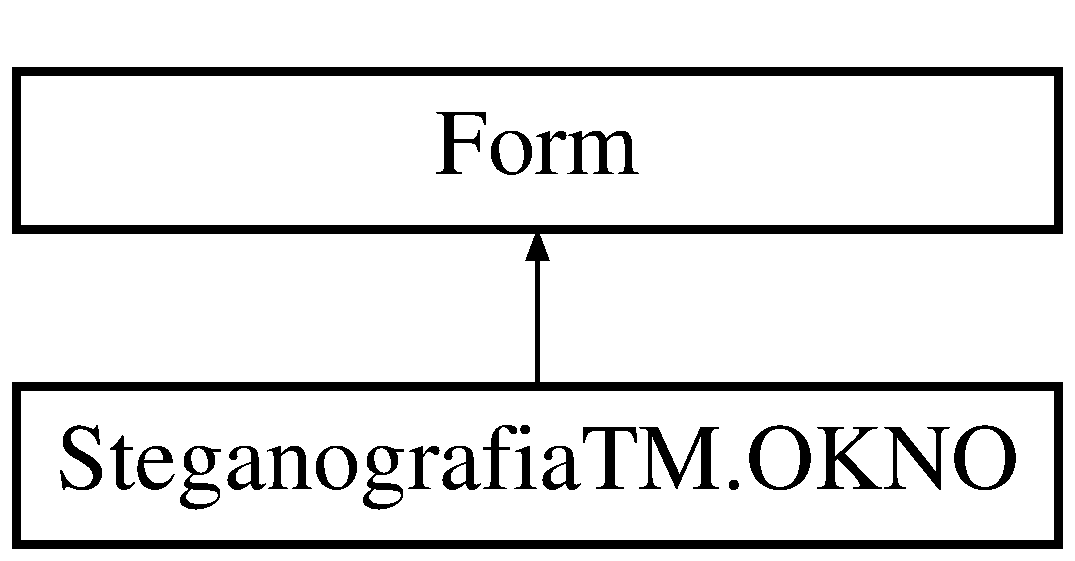
\includegraphics[height=2.000000cm]{class_steganografia_t_m_1_1_o_k_n_o}
\end{center}
\end{figure}
\subsection*{Metody publiczne}
\begin{DoxyCompactItemize}
\item 
\hyperlink{class_steganografia_t_m_1_1_o_k_n_o_af2d455dfcaa09555d6e4eee1a7ab4d06}{O\+K\+NO} ()
\end{DoxyCompactItemize}
\subsection*{Metody chronione}
\begin{DoxyCompactItemize}
\item 
override void \hyperlink{class_steganografia_t_m_1_1_o_k_n_o_aab165c92013c9cd58f51cf2ae5be4531}{Dispose} (bool disposing)
\begin{DoxyCompactList}\small\item\em Clean up any resources being used. \end{DoxyCompactList}\end{DoxyCompactItemize}


\subsection{Opis szczegółowy}


Definicja w linii 13 pliku O\+K\+N\+O.\+cs.



\subsection{Dokumentacja konstruktora i destruktora}
\mbox{\Hypertarget{class_steganografia_t_m_1_1_o_k_n_o_af2d455dfcaa09555d6e4eee1a7ab4d06}\label{class_steganografia_t_m_1_1_o_k_n_o_af2d455dfcaa09555d6e4eee1a7ab4d06}} 
\index{Steganografia\+T\+M\+::\+O\+K\+NO@{Steganografia\+T\+M\+::\+O\+K\+NO}!O\+K\+NO@{O\+K\+NO}}
\index{O\+K\+NO@{O\+K\+NO}!Steganografia\+T\+M\+::\+O\+K\+NO@{Steganografia\+T\+M\+::\+O\+K\+NO}}
\subsubsection{\texorpdfstring{O\+K\+N\+O()}{OKNO()}}
{\footnotesize\ttfamily Steganografia\+T\+M.\+O\+K\+N\+O.\+O\+K\+NO (\begin{DoxyParamCaption}{ }\end{DoxyParamCaption})\hspace{0.3cm}{\ttfamily [inline]}}



Definicja w linii 18 pliku O\+K\+N\+O.\+cs.



\subsection{Dokumentacja funkcji składowych}
\mbox{\Hypertarget{class_steganografia_t_m_1_1_o_k_n_o_aab165c92013c9cd58f51cf2ae5be4531}\label{class_steganografia_t_m_1_1_o_k_n_o_aab165c92013c9cd58f51cf2ae5be4531}} 
\index{Steganografia\+T\+M\+::\+O\+K\+NO@{Steganografia\+T\+M\+::\+O\+K\+NO}!Dispose@{Dispose}}
\index{Dispose@{Dispose}!Steganografia\+T\+M\+::\+O\+K\+NO@{Steganografia\+T\+M\+::\+O\+K\+NO}}
\subsubsection{\texorpdfstring{Dispose()}{Dispose()}}
{\footnotesize\ttfamily override void Steganografia\+T\+M.\+O\+K\+N\+O.\+Dispose (\begin{DoxyParamCaption}\item[{bool}]{disposing }\end{DoxyParamCaption})\hspace{0.3cm}{\ttfamily [inline]}, {\ttfamily [protected]}}



Clean up any resources being used. 


\begin{DoxyParams}{Parametry}
{\em disposing} & true if managed resources should be disposed; otherwise, false.\\
\hline
\end{DoxyParams}


Definicja w linii 14 pliku O\+K\+N\+O.\+Designer.\+cs.



Dokumentacja dla tej klasy została wygenerowana z plików\+:\begin{DoxyCompactItemize}
\item 
Techniki-\/multimedialne-\/\+Projekt-\/\+Steganografia/\+Steganografia\+T\+M C\#/\+Steganografia\+T\+M/\hyperlink{_o_k_n_o_8cs}{O\+K\+N\+O.\+cs}\item 
Techniki-\/multimedialne-\/\+Projekt-\/\+Steganografia/\+Steganografia\+T\+M C\#/\+Steganografia\+T\+M/\hyperlink{_o_k_n_o_8_designer_8cs}{O\+K\+N\+O.\+Designer.\+cs}\end{DoxyCompactItemize}

\chapter{Dokumentacja plików}
\hypertarget{_kodowanie_8cs}{}\section{Dokumentacja pliku Techniki-\/multimedialne-\/\+Projekt-\/\+Steganografia/\+Steganografia\+TM C\#/\+Steganografia\+T\+M/\+Kodowanie.cs}
\label{_kodowanie_8cs}\index{Techniki-\/multimedialne-\/\+Projekt-\/\+Steganografia/\+Steganografia\+T\+M C\#/\+Steganografia\+T\+M/\+Kodowanie.\+cs@{Techniki-\/multimedialne-\/\+Projekt-\/\+Steganografia/\+Steganografia\+T\+M C\#/\+Steganografia\+T\+M/\+Kodowanie.\+cs}}
\subsection*{Przestrzenie nazw}
\begin{DoxyCompactItemize}
\item 
namespace \hyperlink{namespace_steganografia_t_m}{Steganografia\+TM}
\end{DoxyCompactItemize}

\hypertarget{_o_k_n_o_8cs}{}\section{Dokumentacja pliku Techniki-\/multimedialne-\/\+Projekt-\/\+Steganografia/\+Steganografia\+TM C\#/\+Steganografia\+T\+M/\+O\+K\+NO.cs}
\label{_o_k_n_o_8cs}\index{Techniki-\/multimedialne-\/\+Projekt-\/\+Steganografia/\+Steganografia\+T\+M C\#/\+Steganografia\+T\+M/\+O\+K\+N\+O.\+cs@{Techniki-\/multimedialne-\/\+Projekt-\/\+Steganografia/\+Steganografia\+T\+M C\#/\+Steganografia\+T\+M/\+O\+K\+N\+O.\+cs}}
\subsection*{Struktury danych}
\begin{DoxyCompactItemize}
\item 
class \hyperlink{class_steganografia_t_m_1_1_o_k_n_o}{Steganografia\+T\+M.\+O\+K\+NO}
\end{DoxyCompactItemize}
\subsection*{Przestrzenie nazw}
\begin{DoxyCompactItemize}
\item 
namespace \hyperlink{namespace_steganografia_t_m}{Steganografia\+TM}
\end{DoxyCompactItemize}

\hypertarget{_o_k_n_o_8_designer_8cs}{}\section{Dokumentacja pliku Techniki-\/multimedialne-\/\+Projekt-\/\+Steganografia/\+Steganografia\+TM C\#/\+Steganografia\+T\+M/\+O\+K\+NO.Designer.\+cs}
\label{_o_k_n_o_8_designer_8cs}\index{Techniki-\/multimedialne-\/\+Projekt-\/\+Steganografia/\+Steganografia\+T\+M C\#/\+Steganografia\+T\+M/\+O\+K\+N\+O.\+Designer.\+cs@{Techniki-\/multimedialne-\/\+Projekt-\/\+Steganografia/\+Steganografia\+T\+M C\#/\+Steganografia\+T\+M/\+O\+K\+N\+O.\+Designer.\+cs}}
\subsection*{Struktury danych}
\begin{DoxyCompactItemize}
\item 
class \hyperlink{class_steganografia_t_m_1_1_o_k_n_o}{Steganografia\+T\+M.\+O\+K\+NO}
\end{DoxyCompactItemize}
\subsection*{Przestrzenie nazw}
\begin{DoxyCompactItemize}
\item 
namespace \hyperlink{namespace_steganografia_t_m}{Steganografia\+TM}
\end{DoxyCompactItemize}

\hypertarget{_program_8cs}{}\section{Dokumentacja pliku Techniki-\/multimedialne-\/\+Projekt-\/\+Steganografia/\+Steganografia\+TM C\#/\+Steganografia\+T\+M/\+Program.cs}
\label{_program_8cs}\index{Techniki-\/multimedialne-\/\+Projekt-\/\+Steganografia/\+Steganografia\+T\+M C\#/\+Steganografia\+T\+M/\+Program.\+cs@{Techniki-\/multimedialne-\/\+Projekt-\/\+Steganografia/\+Steganografia\+T\+M C\#/\+Steganografia\+T\+M/\+Program.\+cs}}
\subsection*{Komponenty}
\begin{DoxyCompactItemize}
\item 
class {\bfseries Steganografia\+T\+M.\+Program}
\end{DoxyCompactItemize}
\subsection*{Przestrzenie nazw}
\begin{DoxyCompactItemize}
\item 
namespace \hyperlink{namespace_steganografia_t_m}{Steganografia\+TM}
\end{DoxyCompactItemize}

%--- End generated contents ---

% Index
\backmatter
\newpage
\phantomsection
\clearemptydoublepage
\addcontentsline{toc}{chapter}{Indeks}
\printindex

\end{document}
